\documentclass[12pt]{article}
\usepackage[margin=1in]{geometry}
\usepackage{graphicx}
\usepackage{booktabs}
\usepackage{amsmath}
\usepackage{amssymb}
\usepackage{float}
\usepackage{caption}
\usepackage{setspace}
\usepackage[most]{tcolorbox}
\captionsetup{font=small, labelfont=bf, skip=6pt}
\onehalfspacing

\newtcolorbox{explain}{%
  colback=black!3,
  colframe=black!25,
  boxrule=0.5pt,
  arc=1pt,
  left=8pt,
  right=8pt,
  top=5pt,
  bottom=5pt,
  before skip=6pt,
  after skip=12pt,
  fontupper=\normalsize
}

\title{Evaluation Protocol Freeze\\[0.2em]
\large Bitcoin realized volatility}
\author{Volatility forecasting project}
\date{29 September 2026}

\begin{document}
\maketitle

\noindent
This step \textbf{only freezes} the out-of-sample protocol.
No HAR / ARIMA / GARCH / LSTM fitting belongs here.
Code: \texttt{eval\_freeze/protocol.py}. Sanity check runner: \texttt{eval\_freeze/run\_freeze.py}.

\section{What is frozen}
\begin{itemize}
  \item Target: \(y_t=\log\mathrm{RV}_{t+1}\)
  \item Chronological train / val / test cuts (no shuffle)
  \item Protocol B: tune, then \textbf{refit on train+val}, score on test
  \item Metrics: RMSE and MAE on log-RV; QLIKE on RV
  \item Val usage: LSTM tuning / early stopping only
\end{itemize}
\begin{explain}
Later steps import these helpers. They must not redefine splits or metrics.
Classical series model on \(\log\mathrm{RV}\) is ARIMA. Multi-horizon persistence is handled by HAR; the ARIMA baseline is a low-order fit on the same \(\log\mathrm{RV}\) series.
\end{explain}

\section{Target}
\[
y_t=\log\mathrm{RV}_{t+1},
\qquad
\mathrm{RV}_{t+1}=\exp(y_t).
\]
\begin{explain}
Log-RV models forecast \(\hat y_t\). GARCH forecasts \(\hat\sigma_{t+1}\) and is scored against the same realized \(\mathrm{RV}_{t+1}\) on the same test dates.
\end{explain}

\section{Chronological splits (Protocol B)}
\begin{table}[H]
\centering
\begin{tabular}{llrr}
\toprule
Split & Role in this protocol & Dates (UTC) & \(n\) \\
\midrule
Train & Tuning-stage fit & 17 Sep 2017 -- 31 Dec 2021 & 1{,}540 \\
Val & LSTM tune / early stop only & 1 Jan 2022 -- 31 Dec 2023 & 729 \\
Train+Val & Final fit before test & 17 Sep 2017 -- 31 Dec 2023 & 2{,}269 \\
Test & Leaderboard metrics only & 1 Jan 2024 -- 25 Sep 2026 & 999 \\
\bottomrule
\end{tabular}
\caption{Frozen calendar.}
\end{table}
\begin{figure}[H]
\centering
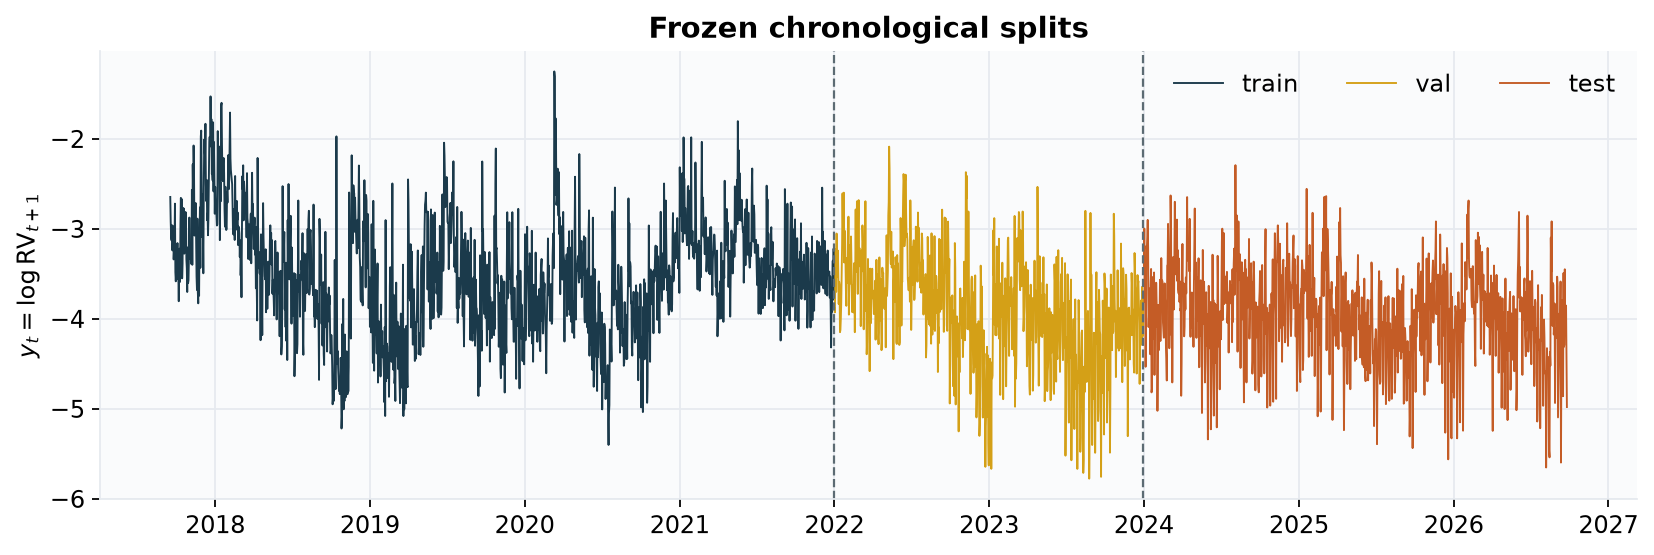
\includegraphics[width=\textwidth]{figures/splits_timeline.png}
\caption{Target path colored by split.}
\end{figure}
\begin{explain}
Workflow: (1) tune on train (+ val for LSTM); (2) refit on train+val with frozen choices; (3) score on test.
Helper: \texttt{fit\_mask(..., stage='tune'|'final')}.
\end{explain}

\section{Metrics}
\[
\mathrm{RMSE}=\sqrt{\frac1n\sum (y_t-\hat y_t)^2},
\qquad
\mathrm{MAE}=\frac1n\sum |y_t-\hat y_t|,
\]
\[
\mathrm{QLIKE}
=
\frac1n\sum_t
\Biggl(
\frac{\mathrm{RV}_{t+1}}{\widehat{\mathrm{RV}}_{t+1}}
-
\ln\frac{\mathrm{RV}_{t+1}}{\widehat{\mathrm{RV}}_{t+1}}
-1
\Biggr).
\]
\begin{explain}
RMSE/MAE use the log-RV scale. QLIKE uses \(\widehat{\mathrm{RV}}=\exp(\hat y)\) or GARCH \(\hat\sigma\).
AIC may be used later when picking ARIMA/GARCH \emph{orders} on train; AIC is not a leaderboard metric.
\end{explain}

\section{Protocol sanity check (not a baseline step)}
A parameter-free lag-1 rule \(\hat y_t=\log\mathrm{RV}_t\) is run only to verify splits and metric code.
Full baselines (Naive as a named model, HAR, ARIMA, GARCH, \ldots) start in the next step.
\begin{figure}[H]
\centering
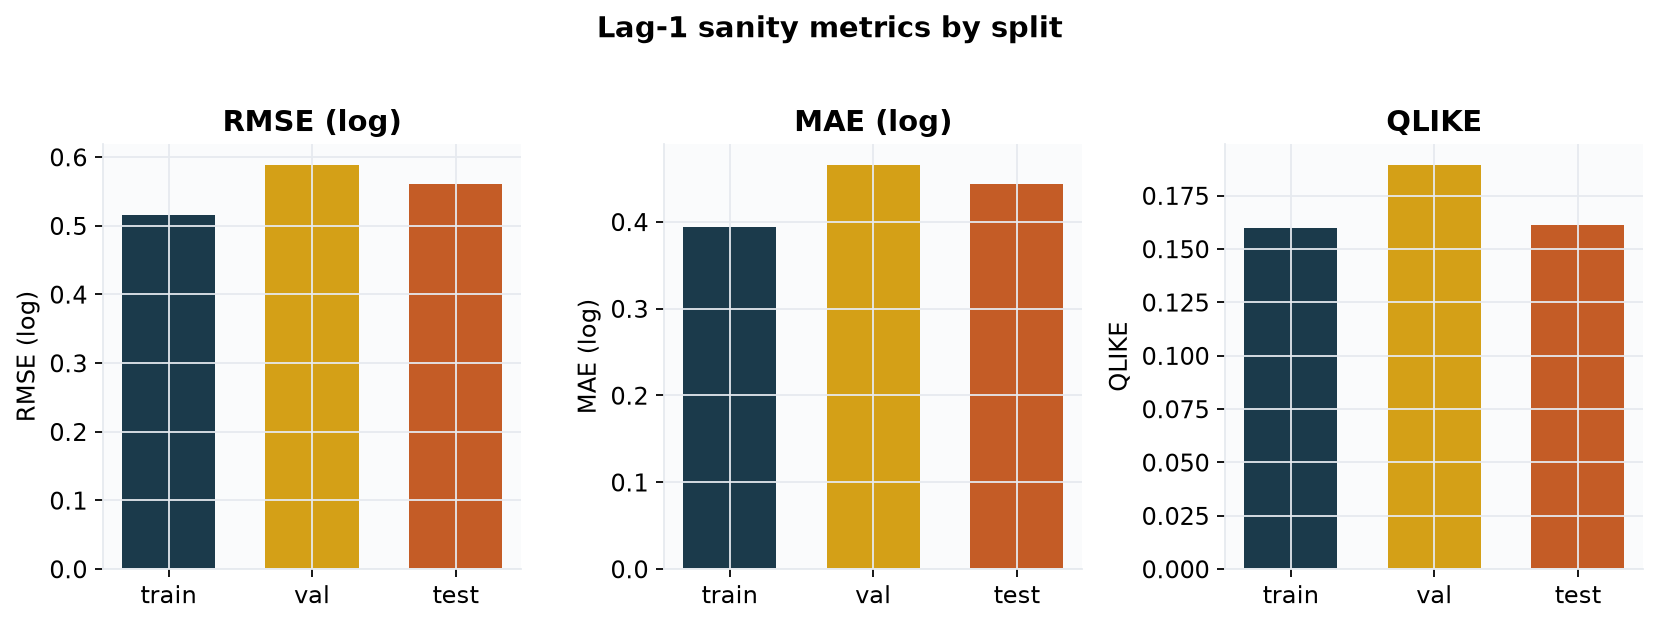
\includegraphics[width=\textwidth]{figures/naive_metrics.png}
\caption{Sanity metrics by split for the lag-1 rule.}
\end{figure}
\begin{table}[H]
\centering
\begin{tabular}{lccc}
\toprule
Split & RMSE (log) & MAE (log) & QLIKE \\
\midrule
Train & 0.516 & 0.394 & 0.160 \\
Val & 0.589 & 0.466 & 0.190 \\
Test & 0.560 & 0.444 & 0.161 \\
\bottomrule
\end{tabular}
\caption{Lag-1 sanity numbers (test is the future leaderboard floor).}
\end{table}

\section{Artifacts}
\begin{itemize}
  \item \texttt{eval\_freeze/protocol.py}
  \item \texttt{eval\_freeze/splits.parquet}
  \item \texttt{eval\_freeze/freeze\_stats.json}
\end{itemize}

\section{Synthesis}
Protocol B is frozen under \texttt{eval\_freeze/}.
This step does not fit forecasting models.
Next: baselines under the same splits and metrics (Naive, HAR, ARIMA, GARCH-family).

\end{document}
